\documentclass[12pt,a4paper,oneside]{book}

\usepackage[utf8]{inputenc}
\usepackage[english]{babel}
\usepackage{amssymb}
\usepackage{frontespizio}
\usepackage{enumitem}
\usepackage{fancyhdr}
\usepackage{eurosym}
\usepackage{graphicx}
\usepackage{xcolor}
\usepackage{minted}

\fancypagestyle{plain}{
	\fancyhf{}
	\fancyfoot[C]{\thepage}
	\renewcommand{\headrulewidth}{\ifnum\value{chapter}>0 0.5pt \else 0pt \fi}
	\renewcommand{\footrulewidth}{0pt}
	\fancyhead[L]{\ifnum\value{chapter}>0 \bfseries \itshape \nouppercase \leftmark \fi}
}

\pagestyle{plain}

\newcommand\itemtext[2]{
	\expandafter\gdef\csname item#1\endcsname{#2}
	\label{#1}#2}

\newcommand\refitemtext[1]{\csname item#1\endcsname}

\begin{document}
	
\begin{frontespizio}
	\Istituzione{Politecnico di Milano}
	\Logo[3cm]{logo.png}
	\Divisione{Computer Science and Engineering}
	\Scuola{}
	\Titoletto{Software Engineering 2}
	\Titolo{Code Inspection}
	\Sottotitolo{\textbf{PowerEnJoy}}
	\NCandidato{Authors}
	\Candidato{Francesco Fabiani\\Jagadesh Manivannan\\Niccolò Pozzolini}
	\NRelatore{Professors}{}
	\Relatore{Elisabetta Di Nitto\\Luca Mottola}
	\Annoaccademico{2016}
	\Piede{Version 1.0 \kern7cm February 5\(\mathbf{^{th}}\) 2017}
\end{frontespizio}
 
\tableofcontents

\chapter{Introduction}

\section{Description of the given problem}
\section{Goals}
\section{Domain properties}
\section{Glossary}
\section{Constrains}
\section{Proposed system}
\section{Reference documents}
\chapter{Architectural design}

\section{Overview}

\section{Component view}

\section{Deployment view}
\begin{figure}[t]
	\centering
	\includegraphics[height=6.7cm,keepaspectratio]{figures/deployment_view.eps}
	\caption{Use case diagram for PowerEnJoy}
	\label{fig:deployment_view}
\end{figure}

\section{Runtime view}

\section{Component interfaces}

\section{Selected architectural styles and patterns}

\section{Other design decisions}

\chapter{Algorithm design}

In this chapter we are going to present two of the algorithms thought for our system. The language used to describe them is based on Java, with the sporadic addition of pseudocode and comments for the least interesting parts of the code.

\section{Discounts and penalties}
\begin{minted}[tabsize=4,breaklines=true]{java}
Double discountsAndPenalties(Double rideCost) {
	Double discount = 0.0, penalty = 0.0;
	
	if (totalPassengers >= 3) {
		discount = 0.1; // 10% discount
	}
	
	if (batteryStatus >= 0.5) {
		discount = 0.2; // 20% discount
	}
	
	if (car.isCharging()) {
		discount = 0.3; // 30% discount
	}
	
	rideCost -= rideCost * discount;
	
	// distances are expressed in meters
	Double currentDistance, minDistance = Double.MAX_VALUE;
	for (PowerStation ps : PowerStation.listAll()) {
		currentDistance = distance(car.getPosition(), ps.getPosition());
		if (currentDistance < minDistance) {
			minDistance = currentDistance;
		}
	}
	
	if (minDistance > 3000 || batteryStatus < 0.2) {
		penalty = 0.3; // 30% penalty
	}
	
	rideCost += rideCost * penalty;
	
	return rideCost;
}
\end{minted}

\section{Money Saving Option}
\begin{minted}[tabsize=4,breaklines=true]{java}
PowerStation moneySavingOption(Position destination) {
	long[] density;
	int[] distances;
	PowerStation[] stations;
	int distance;
	
	for (i = 0; i < zone.size; i++) {
		density(i) = zone[i].parkedCar.size / zone[i].area;
	}
	
	for (i = 0; i < zone.size; i++) {
		distance = distance(zone[i], destination);
		
		if (avg(density) - density(i) > threshold1 && distance < threshold2) {
			distances.add(distance);
		}
	}
	
	return stations[indexOf(min(distances))];
}
\end{minted}
\chapter{User interface design}

\section{Mock-ups}
We have already presented the mock-ups for mobile and desktop versions of the app in section 2.2.1 of the Requirements analysis and specification document.

\section{UX diagrams}
In this section UX diagrams for some of the relevant operations will be showed in order to better describe the user interaction with the system.

\begin{figure}[h]
	\centering
	\includegraphics[width=6cm,keepaspectratio]{figures/resv_ux_diagram.eps}
	\caption{UX user with active reservation}
	\label{fig:resv_ux_diagram}
\end{figure}

\begin{figure}[h]
	\centering
	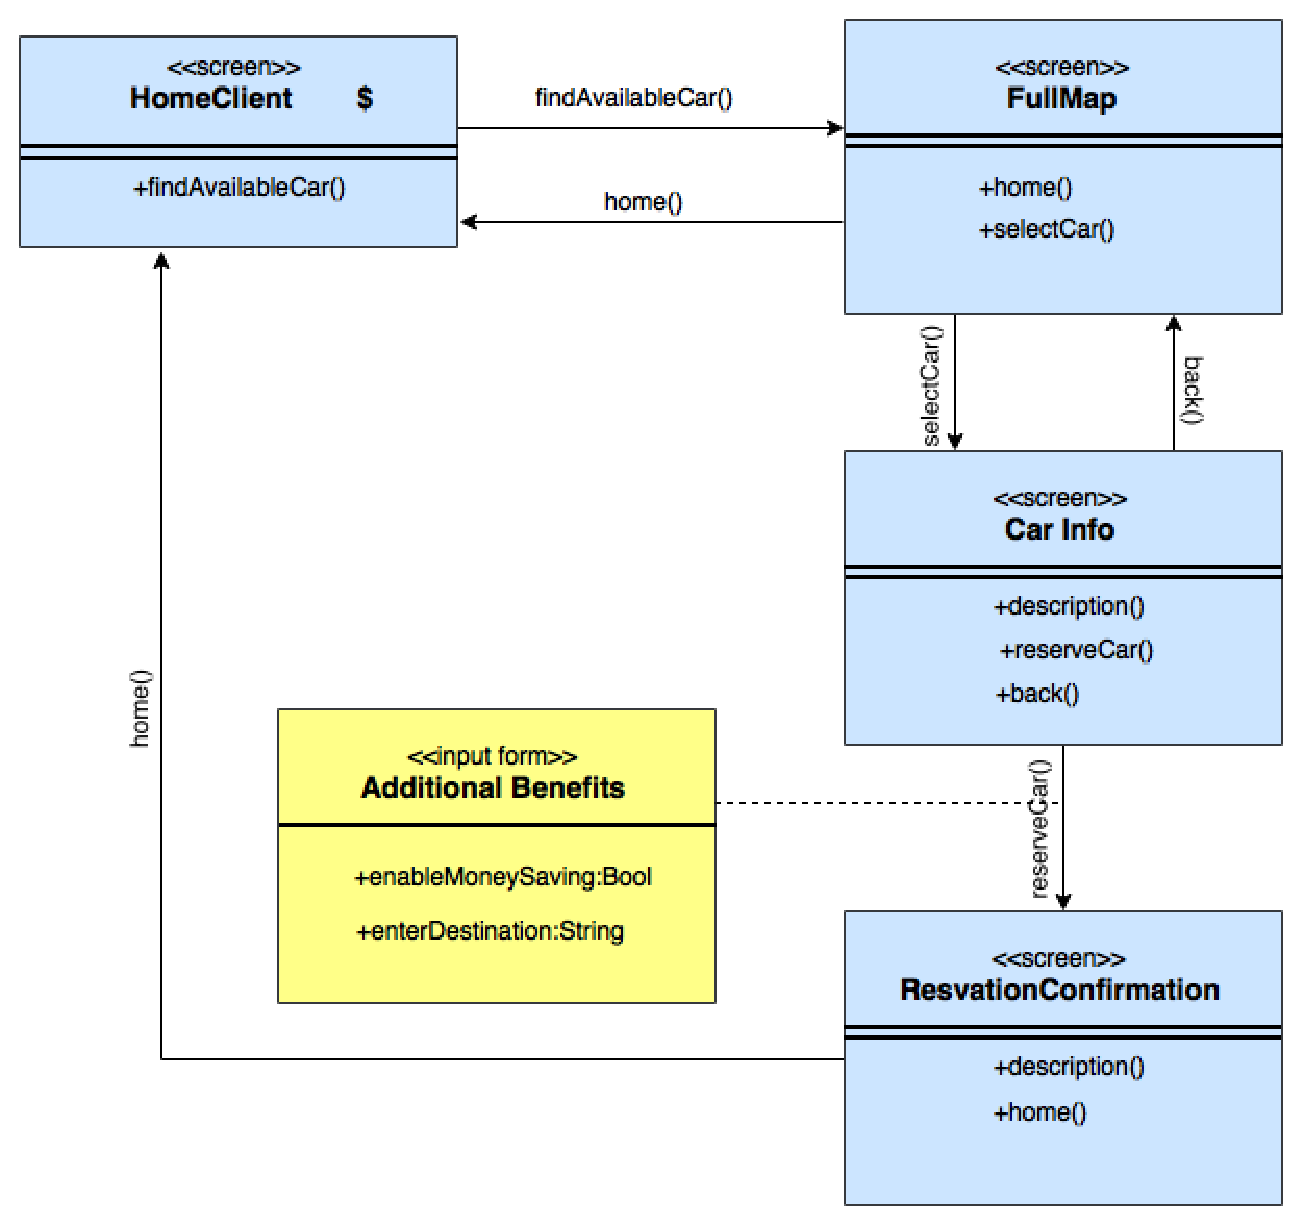
\includegraphics[width=\linewidth,keepaspectratio]{figures/notresv_ux_diagram.eps}
	\caption{UX user with no reservation}
	\label{fig:notresv_ux_diagram}
\end{figure}

\clearpage
\section{BCE diagram}
The figure~\ref{fig:bce_diagram} shows the Business-Controller-Entity diagram for users that access to the homepage not having an active reservation of a car. A BCE diagram is very useful when the MVC pattern is used as arch
\begin{figure}[h]
	\centering
	\includegraphics[height=14cm,keepaspectratio]{figures/bce_diagram.eps}
	\caption{BCE user with no reservation}
	\label{fig:bce_diagram}
\end{figure}
\chapter{Requirements traceability}

Each requirement described in the RASD maps to some of the components reported in this document; below the reader will find the list of components involved for every goal of our service.

\begin{itemize}
	\item {[}G1{]} Registration of a user to the system
	\begin{itemize}
		\item Login Manager
	\end{itemize}

	\item {[}G2{]} Finding the locations of the available cars
	\begin{itemize}
		\item Map Manager
		\item Availability Helper
		\item Cars
	\end{itemize}

	\item {[}G3{]} Reservation of a car
	\begin{itemize}
		\item Map Manager
		\item Selection Manager
		\item Reservation Manager
		\item Reservation Controller
		\item Availability Helper
		\item Cars
	\end{itemize}

	\item {[}G4{]} Expiration of reservation and penalization
	\begin{itemize}
		\item Map Manager
		\item Selection Manager
		\item Reservation Manager
		\item Reservation Controller
		\item Availability Helper
		\item Discount and Penalty Manager
		\item Discount and Penalty Controller
	\end{itemize}

	\item {[}G5{]} Entry of registered user into the car
	\begin{itemize}
		\item Map Manager
		\item Ride Manager
		\item Ride Controller
		\item Car
	\end{itemize}

	\item {[}G6{]} Start charging and notifying the registered user
	\begin{itemize}
		\item Map Manager
		\item Ride Manager
		\item Ride Controller
		\item Discount and Penalty Manager
		\item Discount and Penalty Controller
		\item SMS Gateway Interface
		\item SMS Gateway
	\end{itemize}

	\item {[}G7{]} Stop charging the registered user and lock the
	\begin{itemize}
		\item Map Manager
		\item Ride Manager
		\item Ride Controller
		\item Parking Manager
		\item Parking Controller
		\item Discount and Penalty Manager.
		\item Discount and Penalty Controller
	\end{itemize}

	\item {[}G8{]} Safe areas for parking the reserved cars
	\begin{itemize}
		\item Map Manager
		\item Ride Manager
		\item Ride Controller
		\item Parking Manager
		\item Parking Controller
	\end{itemize}

	\item {[}G9{]} Detection of extra passengers and applying discount
	\begin{itemize}
		\item Map Manager
		\item Ride Manager
		\item Ride Controller
		\item Discount and Penalty Manager
		\item Discount and Penalty Controller
	\end{itemize}

	\item {[}G10{]} Detection of the battery status and applying discount
	\begin{itemize}
		\item Map Manager
		\item Ride Manager
		\item Ride Controller
		\item Discount and Penalty Manager
		\item Discount and Penalty Controller
	\end{itemize}

	\item {[}G11{]} Detection of special parking areas and applying discount
	\begin{itemize}
		\item Map Manager
		\item Ride Manager
		\item Ride Controller
		\item Parking Manager
		\item Parking Controller
		\item Discount and Penalty Manager
		\item Discount and Penalty Controller
	\end{itemize}

	\item {[}G12{]} Checking parking and battery constraints and penalization
	\begin{itemize}
		\item Map Manager
		\item Ride Manager
		\item Ride Controller
		\item Parking Manager
		\item Parking Controller
		\item Discount and Penalty Manager
		\item Discount and Penalty Controller
	\end{itemize}
\end{itemize}
\chapter{Effort spent}

\section{Francesco Fabiani}
\begin{itemize}
	\item 21/11/2016: 1h
	\item 23/11/2016: 2h
	\item 26/11/2016: 1h
	\item 28/11/2016: 1h30min
	\item 30/11/2016: 2h30min
	\item 02/12/2016: 2h
	\item 04/12/2016: 1h30min
	\item 05/12/2016: 2h30min
	\item 06/12/2016: 1h
	\item 07/12/2016: 2h
	\item 08/12/2016: 2h30min
\end{itemize}

\section{Jagadesh Manivannan}
\begin{itemize}
	\item 20/11/2016: 1h30min
	\item 21/11/2016: 1h
	\item 22/11/2016: 1h30min
	\item 24/11/2016: 1h
	\item 25/11/2016: 2h
	\item 27/11/2016: 2h
	\item 29/11/2016: 1h30min
	\item 01/12/2016: 3h
	\item 03/12/2016: 1h30min
	\item 04/12/2016: 2h
	\item 06/12/2016: 2h
	\item 07/12/2016: 1h30min
	\item 09/12/2016: 2h
	\item 10/12/2016: 3h
	\item 11/12/2016: 2h
\end{itemize}

\section{Niccolò Pozzolini}
\begin{itemize}
	\item 21/11/2016: 1h
	\item 22/11/2016: 1h30min
	\item 24/11/2016: 2h
	\item 26/11/2016: 1h30min
	\item 27/11/2016: 2h
	\item 29/11/2016: 2h
	\item 30/11/2016: 2h30min
	\item 02/12/2016: 1h
	\item 03/12/2016: 1h
	\item 04/12/2016: 2h30min
	\item 06/12/2016: 1h
	\item 08/12/2016: 1h
	\item 09/12/2016: 1h30min
	\item 10/12/2016: 2h
	\item 11/12/2016: 2h30min
\end{itemize}
\chapter{References}

\section{Used tools}
The tools we used to create this DD document are:

\begin{itemize}
	\item \emph{Creately.com}: for design of sequence diagram of Runtime view,Deployment View.
	\item \emph{Draw.io}: version control for the development of this document.
	\item \emph{GitHub}: for design of the UML diagrams-component view, UX diagram.
	\item \emph{TeXstudio}: drafting of this document.
\end{itemize}
\chapter{Changelog}

\section{v1.1}
\begin{itemize}
	\item Changed the alloy results 
	\item Added world generated diagrams for the relevant predicates
\end{itemize}

\end{document}